%! TEX program = xelatex

\documentclass{report}
\usepackage[UTF8, heading=true]{ctex}
\usepackage{fancyhdr}
\usepackage{tocloft}
\usepackage[margin=1in]{geometry}
\usepackage{metalogo}                   % \XeLaTeX
\usepackage{float}                      % figure H flag
\usepackage{microtype}                  % break long words
\usepackage[bottom]{footmisc}           % force footnote stay bottom
\usepackage{listings}                   % code
\usepackage{xparse}                     % newcommand multiple optional arguments
\usepackage[hidelinks]{hyperref}
\usepackage{tabularx}

% make chapter stay in the same page
\makeatletter
\renewcommand\chapter{\thispagestyle{plain}%
\global\@topnum\z@
\@afterindentfalse
\secdef\@chapter\@schapter}
\makeatother

% settings %%%%%%%%%%%%%%%%%%
%%%%%%%%%%%%%%%%%%%%%%%%%%%%%
\ctexset{
    chapter = {
        format += \flushleft,
        number = \chinese{chapter},
        name = {实验},
    },
    section = {
        format += \flushleft,
    },
    appendix = {
        number = \Alph{chapter},
        name = {附录},
    },
}

\pagestyle{fancy}
\setlength\cftaftertoctitleskip{2em}
\graphicspath{{./res/}}

% defines %%%%%%%%%%%%%%%%%%%
%%%%%%%%%%%%%%%%%%%%%%%%%%%%%
%\newfontfamily\codeF{Fira Code}
\DeclareDocumentCommand{\inputCode}{ O{c} m }{
    {
        \setmainfont{FiraCode Nerd Font}[
            ItalicFont  = FiraCode Nerd Font
        ]
        \lstinputlisting[
            basicstyle=\codeF,
            language=#1,
            tabsize=4,
            showstringspaces=false,
            breaklines=true,
            frame=shadowbox,
            framexleftmargin=10mm,
            rulesepcolor=\color{black},
            basicstyle=\small,
            numbers=left,
        ]{#2}
    }
}

% report content %%%%%%%%%%%%
%%%%%%%%%%%%%%%%%%%%%%%%%%%%%
\begin{document}

\begin{titlepage}
    \addtolength{\topmargin}{1cm}
    \centering
    
\includegraphics[width=0.6\textwidth]{hust.jpg}\par
    \vspace{1cm}
    {\Huge \heiti 操作系统原理实验报告}\par
    \vspace{10cm}
    {
        \large
        \begin{tabular}{r m{8em}}
            \makebox[6em][s]{学生姓名}:& 胡思勖 \\ \cline{2-2}
            \makebox[6em][s]{学号}:& U201514898\\ \cline{2-2}
            \makebox[6em][s]{专业}:& 计算机科学与技术\\ \cline{2-2}
            \makebox[6em][s]{班级}:& 计卓1501\\ \cline{2-2}
            \makebox[6em][s]{指导教师}:& 张杰\\ \cline{2-2}
        \end{tabular}
    }
    \vfill
    2017年12月25日
\end{titlepage}

\setcounter{tocdepth}{1}
\tableofcontents
% Chapter 1 %%%%%%%%%%%%%%%%%
%%%%%%%%%%%%%%%%%%%%%%%%%%%%%
\chapter{进程控制实验}
\label{prt:jin_cheng_kong_zhi_shi_yan_}

\section{实验目的}
\label{sec:shi_yan_mu_de_1}

\begin{enumerate}
    \item 加深对进程的理解,进一步认识并发执行的实质;
    \item 分析进程争用资源现象,学习解决进程互斥的方法;
    \item 掌握Linux进程基本控制;
    \item 掌握Linux系统中的软中断和管道通信。
\end{enumerate}

\section{实验内容}
\label{sec:shi_yan_nei_rong_1}

编写程序,演示多进程并发执行和进程软中断、管道通信。

\begin{itemize}
    \item 父进程使用系统调用pipe( )建立一个管道,然后使用系统调用fork()创建两个子进程,子进程1和子进程2;
    \item 子进程1每隔1秒通过管道向子进程2发送数据: I send you x times. (x初值为1,每次发送后做加一操作),子进程2从管道读出信息,并显示在屏幕上。
    \item 父进程用系统调用signal()捕捉来自键盘的中断信号(即按Ctrl+C键);当捕捉到中断信号后,父进程用系统调用Kill()向两个子进程发出信号,子进程捕捉到信号后分别输出下列信息后终止:\par
        Child Process l is Killed by Parent!\par
        Child Process 2 is Killed by Parent!\par
    \item 父进程等待两个子进程终止后,释放管道并输出如下的信息后终止\par
        Parent Process is Killed!
\end{itemize}

\section{实验设计}
\label{sec:shi_yan_she_ji_1}

\subsection{总体设计}
\label{sub:zong_ti_she_ji_1}

实验通过三个模块实现:父进程模块,子进程模块1和子进程模块2,他们之间的关系如图\ref{fig:exp1module}所示。父进程负责启动两个子进程,捕捉来自终端的SIGINT信号并向子进程发送SIGUSR1信号,子进程负责处理来自父进程的SIGUSR1信号。此外,子进程1每隔一秒向子进程2通过管道发送消息``I send you x times'',子进程2接收到消息后则将其显示在屏幕上。
\begin{figure}[ht]
    \centering
    
\includegraphics[width=0.4\linewidth]{exp1module.png}
    \caption{实验一的三个模块及其关系}
    \label{fig:exp1module}
\end{figure}

\subsection{详细设计}
\label{sub:xiang_xi_she_ji_1}

对于父进程而言,其流程图如图\ref{fig:exp1MainFlowchart}所示。在开始首先设置signal处理函数,使用handlerMain函数来处理signal,然后创建管道,之后尝试fork子进程1和子进程2。在fork的过程中如果出现错误则直接退出程序。在fork成功后关闭父进程的管道(父进程不需要使用管道通信),然后陷入死循环等待用户发送SIGINT信号结束程序。\par
\begin{figure}[ht]
    \centering
    
\includegraphics[width=0.4\linewidth]{exp1MainFlowchart.png}
    \caption{主函数流程}
    \label{fig:exp1MainFlowchart}
\end{figure}

子进程1的流程图如\ref{fig:exp1Proc1Flowchart}所示。在启动后首先设置SIGINT和SIGUSR1的处理函数,讲SIGINT的处理函数设置为SIG\_IGN,忽略掉来自于终端的SIGINT信号(由于在终端中按下Ctrl-C会向前台进程组中的所有进程发送SIGINT信号,而父进程和子进程又默认属于同一个进程组,因此需要子进程忽略掉来自终端的SIGINT),然后将SIGUSR1的处理函数设置为handlerChild1。之后直接进入死循环,每一次循环首先使用sleep函数等待1秒,然后使用write函数向管道中写入``I send you x times''。\par
\begin{figure}[ht]
    \centering
    
\includegraphics[width=0.2\linewidth]{exp1Proc1Flowchart.png}
    \caption{子进程1流程}
    \label{fig:exp1Proc1Flowchart}
\end{figure}

子进程2的流程如图\ref{fig:exp1Proc2Flowchart}所示。类似的,子进程2在启动后使用与子进程1相同的处理方式处理来自终端以及来自父进程的信号,只不过其用于处理SIGUSR1的函数为handlerChild2。然后陷入死循环,在每一次循环中尝试从管道中读取数据,如果读取的数据长度小于0说明读取出错,此时令此程序返回,否则打印读取到的数据到标准输出。
\begin{figure}[ht]
    \centering
    
\includegraphics[width=0.3\linewidth]{exp1Proc2Flowchart.png}
    \caption{子进程2流程}
    \label{fig:exp1Proc2Flowchart}
\end{figure}

对于主进程而言,其用于处理SIGINT的函数handlerMain被触发后首先向子进程1和子进程2发送SIGUSR1信号,然后使用waitpid等待子进程1和子进程2的结束。当子进程1和子进程2结束后,打印``Parent Process is killed'',然后使用exit(0)退出主进程。\par

而子进程1和子进程2的SIGUSR1处理函数则是简单的打印``Child Process x is killed by parent!'',然后使用exit(0)退出进程。其中x为子进程号,子进程1的x为1,子进程2的x为2。

\section{实验过程}
\label{sec:shi_yan_guo_cheng_1}

\subsection{开发环境}
\label{sub:kai_fa_huan_jing_1}

\begin{tabular}{r l}
    操作系统 & Archlinux x86\_64 \\
    编译器 & gcc 7.2.1 \\
    自动编译 & GNU Make 4.2.1 \\
    资源监视器 & htop 2.0.2 \\
\end{tabular}

\subsection{实验步骤}
\label{sub:shi_yan_bu_zou_1}
首先编写源码,然后使用gcc进行编译,编译选项为-Wall -Werror -g -static -std=c++11 -o experiment1.exe。编译完成后得到可执行文件experiment1.exe,然后在终端下执行experiment1.exe。等待若干秒之后按下Ctrl-C,观察程序的输出结果,结果如图\ref{fig:exp1Output}所示。可以看见在6秒时按下了Ctrl-C,在两个子进程结束后父进程结束。

\begin{figure}[ht]
    \centering
    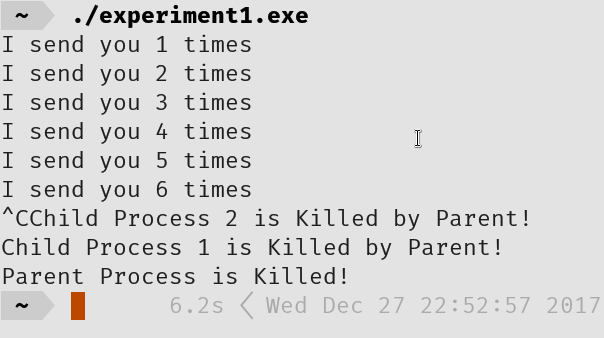
\includegraphics[width=0.7\linewidth]{exp1Output.png}
    \caption{实验一输出结果}
    \label{fig:exp1Output}
\end{figure}

在程序运行时打开htop并进行过滤,可以看到父进程和子进程的关系如\ref{fig:exp1Htop}所示。可以看出程序确实为一个父进程+两个子进程的结构。在htop中分别将SIGINT发送给子进程1和子进程2,程序依旧正常输出,没有任何变化,说明子进程能够正确的忽略掉SIGINT。然后使用SIGUSR1发送给子进程1或子进程2中的任意一个,输出停止,并显示``Child Process x is killed by parent!'',说明能够正确处理SIGUSR1。最后讲SIGTERM发送给父进程,父进程显示``Parent Process is Killed!''后成功退出,与预期结果一致。
\begin{figure}[ht]
    \centering
    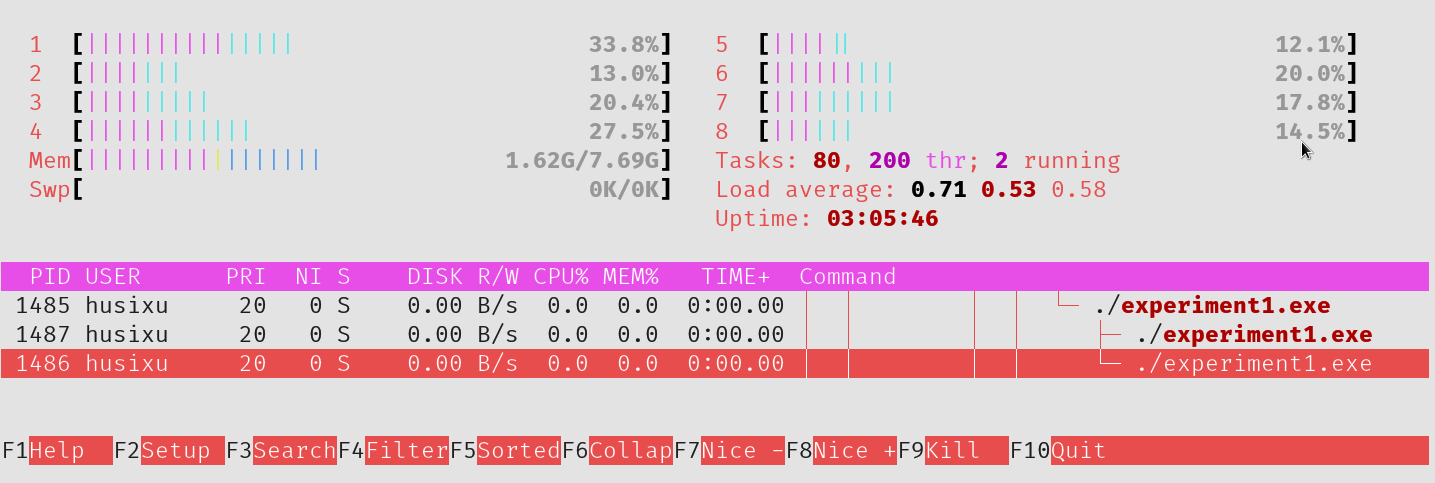
\includegraphics[width=0.9\linewidth]{exp1Htop.png}
    \caption{进程间关系}
    \label{fig:exp1Htop}
\end{figure}

\subsection{结果分析}
\label{sub:jie_guo_fen_xi_}
实验过程中的程序行为与预期一致。通过标准输出可以看出程序确实能够通过管道进行通信,并能够正确的对于信号进行处理,而通过htop中的分别对于各个进程发送信号的结果也验证了这一点,并且也说明了进程之间是能够通过信号进行同步处理的。

% Chapter 2 %%%%%%%%%%%%%%%%%
%%%%%%%%%%%%%%%%%%%%%%%%%%%%%

\chapter{线程同步与通信实验}
\label{cha:xian_cheng_tong_bu_yu_tong_xin_shi_yan_2}

\section{实验目的}
\label{sec:shi_yan_mu_de_2}

\begin{enumerate}
    \item 掌握Linux下线程的概念;
    \item 了解Linux线程同步与通信的主要机制;
    \item 通过信号灯操作实现线程间的同步与互斥。
\end{enumerate}

\section{实验内容}
\label{sec:shi_yan_nei_rong_2}
通过Linux多线程与信号灯机制,设计并实现计算机线程与I/O线程共享缓冲区的同步与通信。\par
程序要求:两个线程,共享公共变量a:\par
\hspace{4em}线程1负责计算(1到100的累加,每次加一个数)\par
\hspace{4em}线程2负责打印(输出累加的中间结果)\par

\section{实验设计}
\label{sec:shi_yan_she_ji_2}

\subsection{总体设计}
\label{sub:zong_ti_she_ji_2}
在此实验的总体设计中,总共使用两个信号量,分别作为线程1计算完成信号和线程2打印完成信号,分别称其为信号量0和信号量1。程序的总体结构如图\ref{fig:exp2Structure}所示。在子线程1在开始时首先对于信号量1进行一次P操作每进行一次累加后作为生产者对信号量0进一次V操作,表示可以开始打印中间结果;线程2在开始前先对信号量0进行P操作,输出结果后再对信号量1进行一次V操作,表示可以进行下一次累加。在累加完成后,线程2等待线程1的结束,主线程等待线程2的结束。

\begin{figure}[ht]
    \centering
    
\includegraphics[width=0.6\linewidth]{exp2Structure.png}
    \caption{程序总体结构}
    \label{fig:exp2Structure}
\end{figure}

\subsection{详细设计}
\label{sub:xiang_xi_she_ji_2}

对于主线程而言,其流程图如图\ref{fig:exp1MainFlowchart}所示,其工作为初始化两个信号量,创建两个线程以及等待线程2的结束,在线程2结束后销毁创建的信号量并结束自身。由于线程2一定在线程1之后结束,因此主线程无需等待线程1的结束。在初始化信号量时,信号量0的初值设置为0,信号量1的初值设置为1,否则线程1无法进入循环,整个程序会死锁。
\begin{figure}[ht]
    \centering
    
\includegraphics[width=0.18\linewidth]{exp2MainFlowchart.png}
    \caption{主线程流程图}
    \label{fig:exp2MainFlowchart}
\end{figure}

线程1的流程图如图\ref{fig:exp2Thread1Flowchart}所示,在每一次循环开始时对信号量1进行P操作,在循环结束时对信号量0进行V操作。此外,在整个循环结束后,将全局变量termFlag设置为1以告知线程2累加操作已经全部结束。
\begin{figure}[ht]
    \centering
    
\includegraphics[width=0.28\linewidth]{exp2Thread1Flowchart.png}
    \caption{线程1流程图}
    \label{fig:exp2Thread1Flowchart}
\end{figure}

线程2的流程图如图\ref{fig:exp2Thread2Flowchart}所示。在每次循环开始时对信号量0进行P操作,在循环结束时对信号量1进行V操作,以达到与线程1的同步。此外,在每次打印后需要检测线程1的循环是否已经完成,即TermFlag是否已经设置,若是,则等待线程1的结束并将自身结束。
\begin{figure}[H]
    \centering
    
\includegraphics[width=0.28\linewidth]{exp2Thread2Flowchart.png}
    \caption{线程2流程图}
    \label{fig:exp2Thread2Flowchart}
\end{figure}

\section{实验过程}
\label{sec:shi_yan_guo_cheng_2}

\subsection{开发环境}
\label{sub:kai_fa_huan_jing_2}

\begin{tabular}{r l}
    操作系统 & Archlinux x86\_64 \\
    编译器 & gcc 7.2.1 \\
    自动编译 & GNU Make 4.2.1 \\
\end{tabular}

\subsection{实验步骤}
\label{sub:shi_yan_bu_zou_2}

编写源码并编译,编译选项为-Wall -Werror -g -static -std=c++11 -o experiment2.exe,编译完成后直接运行得到的experiment2.exe可执行文件并观察输出结果。输出结果如图\ref{fig:exp2ResultProcessed}所示。从结果中可以看出,程序能够正确的运行并能够正确输出每一步的结果。在输出完所有的结果后能够正确的退出,说明程序功能正常。

\begin{figure}[ht]
    \centering
    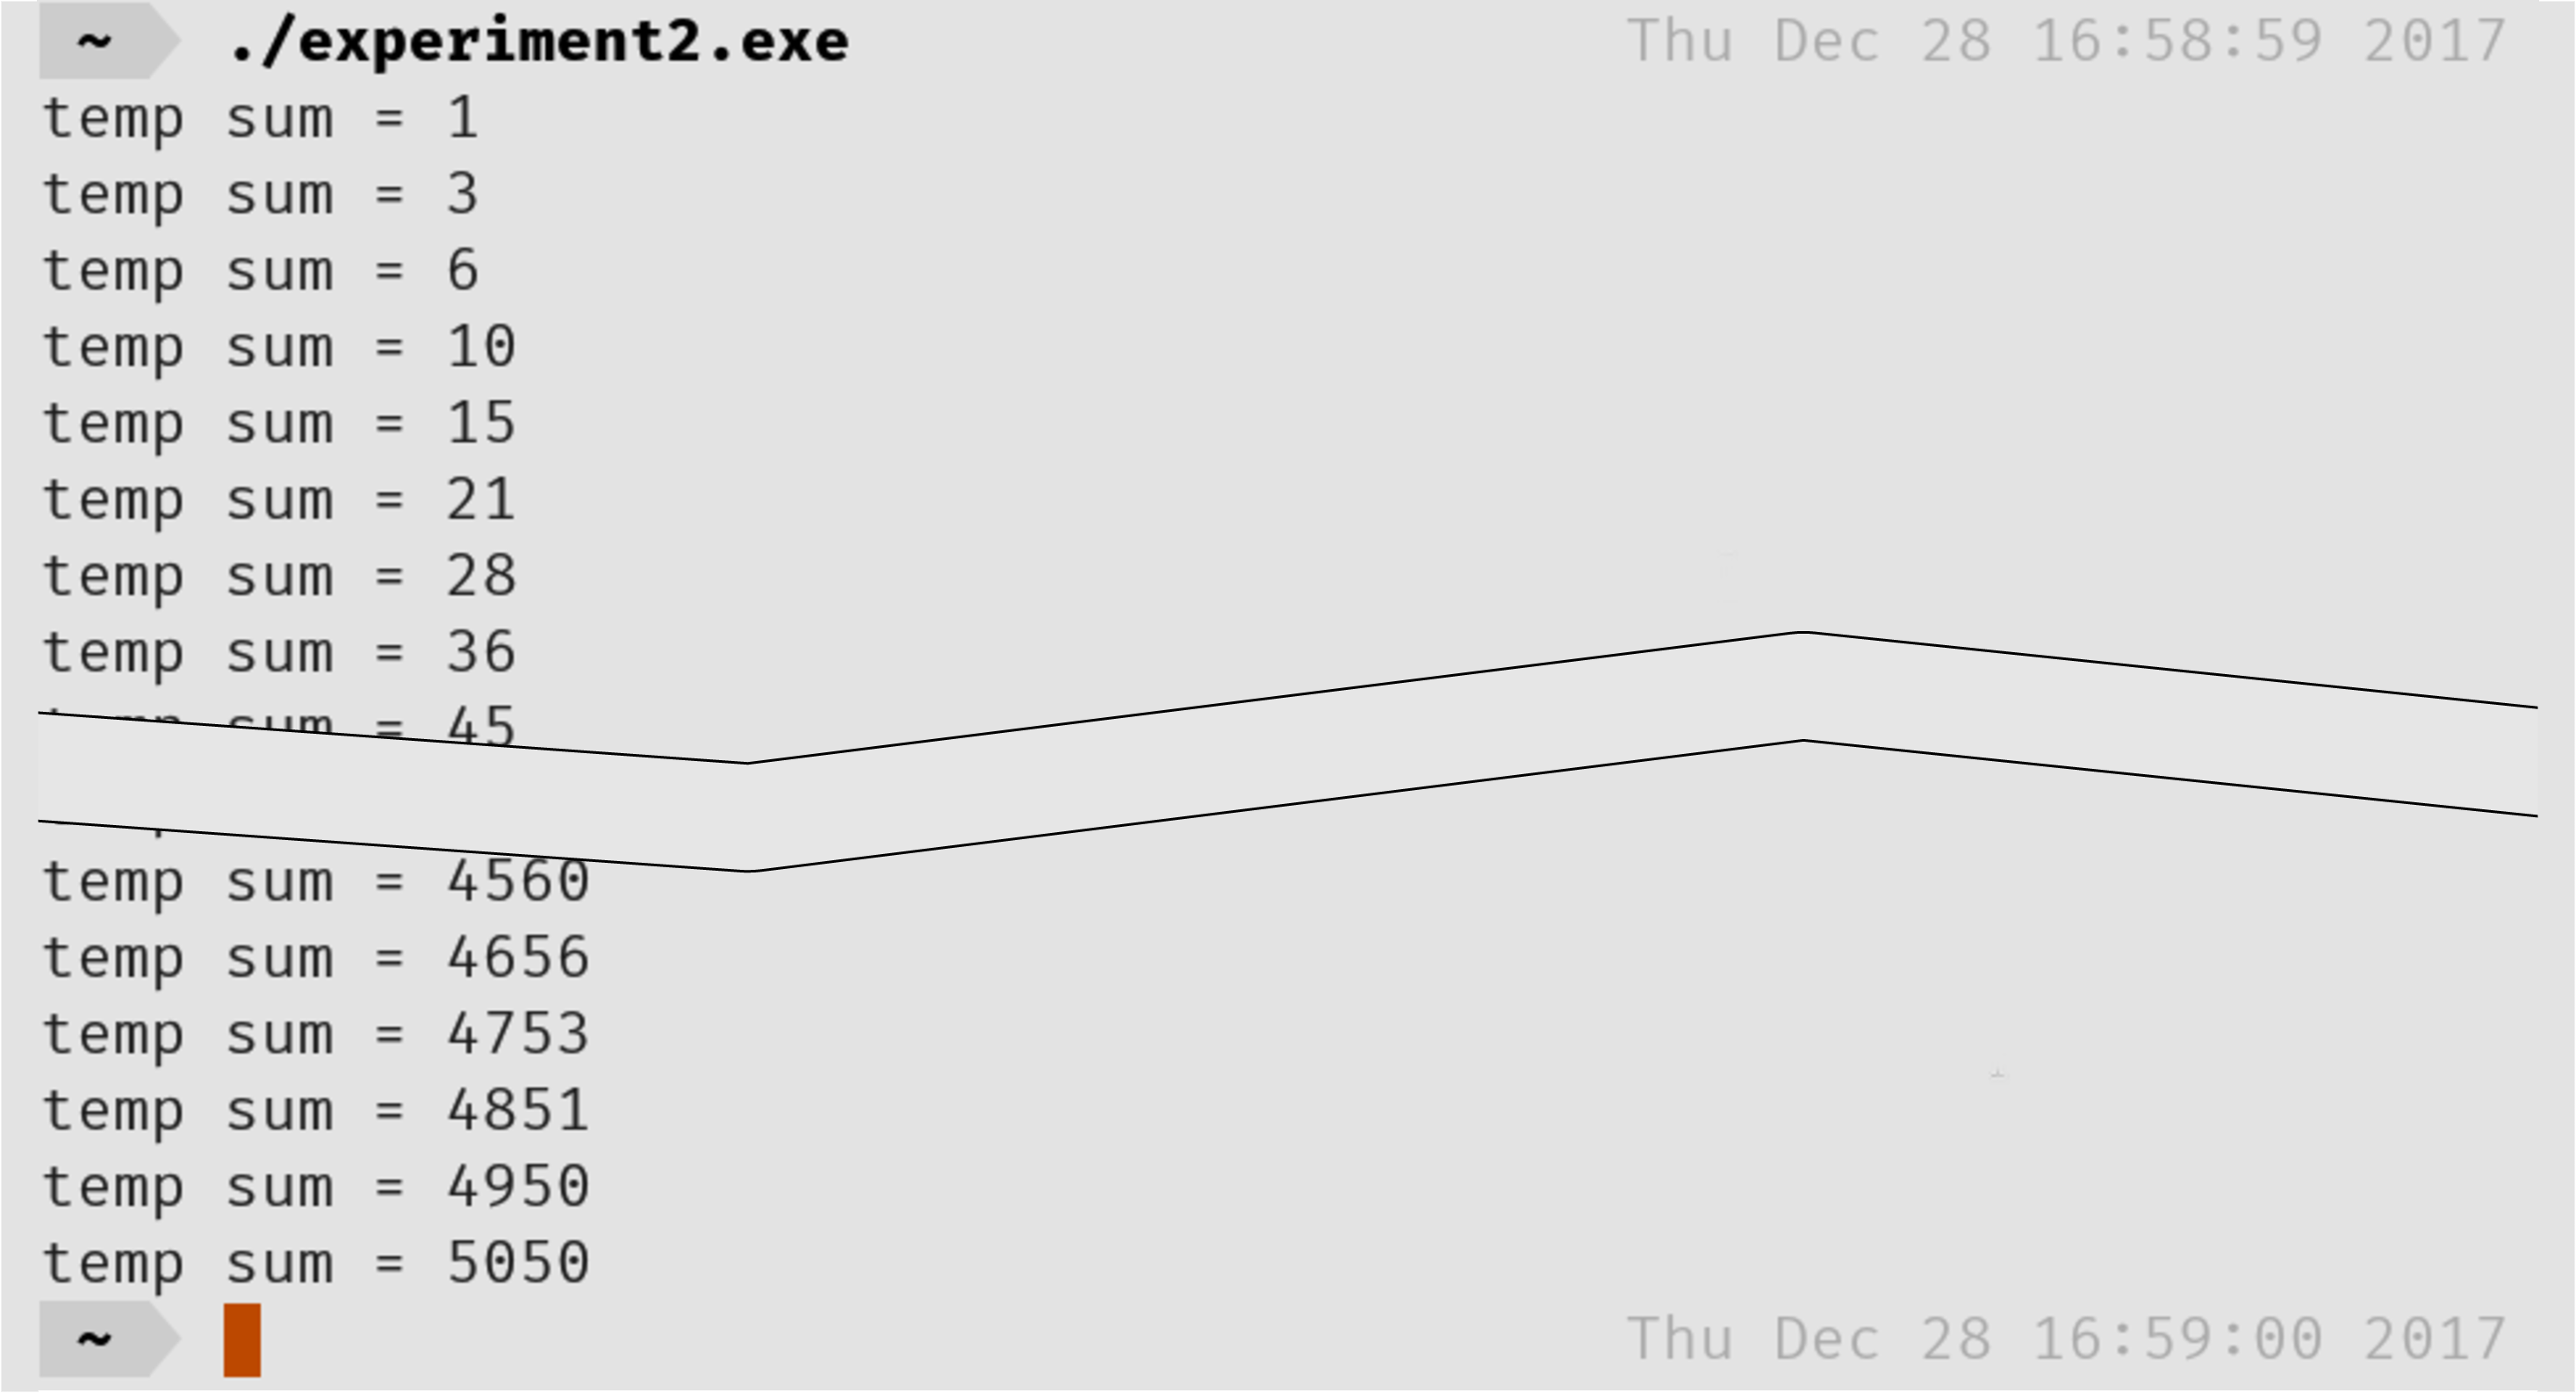
\includegraphics[width=0.8\linewidth]{exp2ResultProcessed.png}
    \caption{程序运行输出结果}
    \label{fig:exp2ResultProcessed}
\end{figure}

在程序没有调试到完全正确之前,出现过输出不连续,输出完成后程序不能结束,或者完全没有输出等错误情况,经过检查后发现是由于没有正确的处理信号量的初值以及生产者--消费者的关系导致的。

\subsection{结果分析}
\label{sub:jie_guo_fen_xi_2}
程序能够对于每一次迭代进行正确的输出,并且程序能够正确的退出,说明程序的逻辑是正常的。这也说明了同一程序的线程之间能够通过信号量进行同步与互斥操作。


% Chapter 3 %%%%%%%%%%%%%%%%%
%%%%%%%%%%%%%%%%%%%%%%%%%%%%%

\chapter{共享内存与进程同步}
\label{cha:xian_cheng_tong_bu_yu_tong_xin_shi_yan_3}

\section{实验目的}
\label{sec:shi_yan_mu_de_3}
\begin{enumerate}
    \item 掌握Linux下共享内存的概念与使用方法;
    \item 掌握环形缓冲的结构与使用方法;
    \item 掌握Linux下进程同步与通信的主要机制。
\end{enumerate}

\section{实验内容}
\label{sec:shi_yan_nei_rong_3}
利用多个共享内存(有限空间)构成的环形缓冲,将源文件复制到目标文件,实现两个进程的誊抄。

\section{实验设计}
\label{sec:shi_yan_she_ji_3}

\subsection{总体设计}
\label{sub:zong_ti_she_ji_3}

整个程序由三个进程构成:主进程、读进程与写进程。主进程用于初始化环形缓冲区、启动两个子进程并等待两个子进程的结束,读进程用于从文件中读取数据并将数据写入环形缓冲区,而写进程则负责从环形缓冲区中读取数据并写入新文件中。线程之间的同步通过三个信号量进行,分别将其称为信号量0、1、2。信号量0用于标识读进程读入的数据量,信号量1用于标识环形缓冲中剩余的空间,信号量2用于进程间的互斥,即同时只允许一个进程访问环形缓冲区。整个程序的结构如\ref{fig:exp3Structure}所示。

\begin{figure}[ht]
    \centering
    
\includegraphics[width=0.4\linewidth]{exp3Structure.png}
    \caption{程序总体结构}
    \label{fig:exp3Structure}
\end{figure}


\subsection{详细设计}
\label{sub:xiang_xi_she_ji_3}

主线程开始时首先尝试打开源文件和目标文件(文件名由命令行传入),成功后尝试创建环形缓冲区,环形缓冲区结构及其每个结点的结构如图\ref{fig:exp3DataStructure}所示,每个节点中包含一个nextShmId指向下一个共享内存区,并包含一个数据区域用于存储数据。在环形缓冲区创建完成后,尝试创建3个信号量,由于信号量0用于表示读入的数据量、信号量1用于表示缓冲区剩余数量,信号量2用于加锁,因此信号量0、1、2的初值分别赋0,环形缓冲区结点个数,1。最后,尝试创建读进程和写进程并等待两个进程结束。在两个进程结束后,释放所有申请的资源。在整个主线程执行的过程中,如果打开文件、创建缓冲区、创建信号量或启动子进程中的任何一步不能成功执行则立即释放已经分配的资源并退出程序。

\begin{figure}[ht]
    \centering
    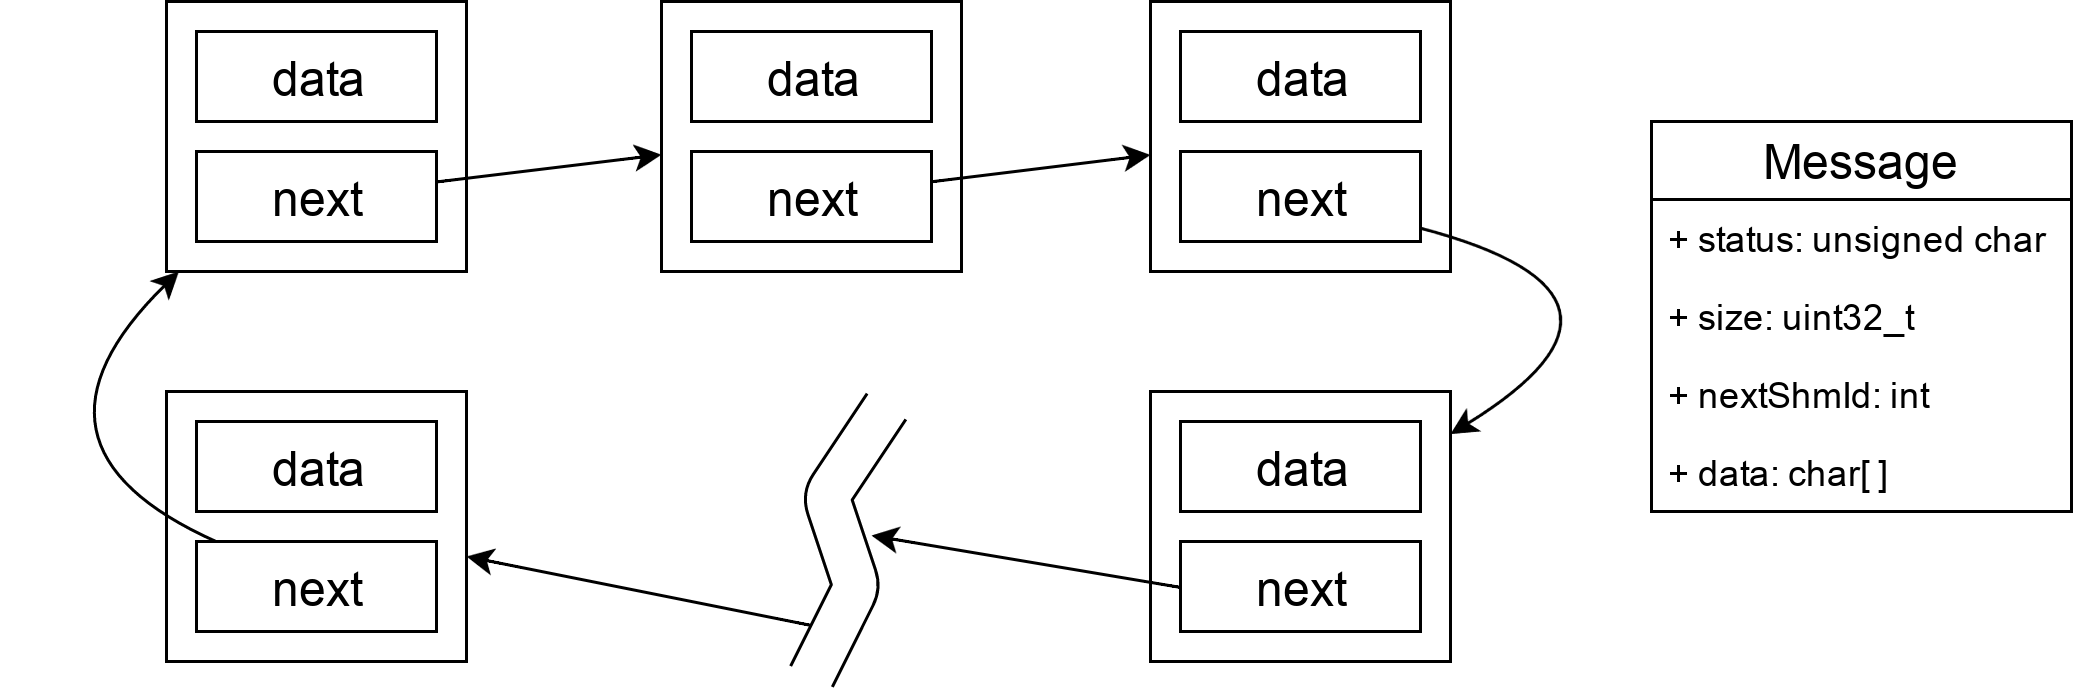
\includegraphics[width=0.7\linewidth]{exp3DataStructure.png}
    \caption{缓冲区及其节点结构}
    \label{fig:exp3DataStructure}
\end{figure}

读文件进程的流程图如图\ref{fig:exp3Proc1Flowchart}所示,进程开始即进入读文件循环,每次循环开始前首先对信号量1和信号量2进行P操作,分别表示从环形缓冲区取得一个节点以及对环形缓冲区加锁。然后读取文件的一个片段,此片段大小为不大于环形缓冲区每个节点数据区的大小(由主进程在初始化环形缓冲区时指定),将其放入环形缓冲区尾部。然后判断是否读到文件尾部,若是,则关闭文件,否则执行下一个循环。在关闭文件或者执行下一个循环之前对于信号量0和信号量2进行V操作,表示增加一个读取的数据以及释放环形缓冲区的锁。
\begin{figure}[H]
    \centering
    
\includegraphics[width=0.3\linewidth]{exp3Proc1Flowchart.png}
    \caption{读文件进程流程}
    \label{fig:exp3Proc1Flowchart}
\end{figure}

写文件进程的流程与读文件进程相似,其流程图图如图\ref{fig:exp3Proc2Flowchart}所示。进程开始后立即进入写文件循环,每次循环开始前首先对于信号量0和信号量2进行P操作,表示从读取的数据片段中取一个片段以及获得环形缓冲区的锁。然后尝试将读取的数据写入文件。写入后判断这一片段是否为读文件进程向环形缓冲区添加的最后一个片段,读文件进程会向环形缓冲区节点的status成员写入这一数据(见图\ref{fig:exp3DataStructure})。如果这一片段是最后一个片段,说明读文件进程已经完成文件读取操作,此时关闭目标文件,否则进行下一个循环。在关闭文件或进行下一个循环前对于信号量1和信号量2进行V操作,表示释放一个空节点到环形缓冲区,以及从释放环形缓冲区的锁。

\begin{figure}[ht]
    \centering
    
\includegraphics[width=0.3\linewidth]{exp3Proc2Flowchart.png}
    \caption{写文件进程流程图}
    \label{fig:exp3Proc2Flowchart}
\end{figure}

\section{实验过程}
\label{sec:shi_yan_guo_cheng_3}

\subsection{开发环境}
\label{sub:kai_fa_huan_jing_3}

\begin{tabular}{r l}
    操作系统 & Archlinux x86\_64 \\
    编译器 & gcc 7.2.1 \\
    自动编译 & GNU Make 4.2.1 \\
\end{tabular}

\subsection{实验步骤}
\label{sub:shi_yan_bu_zou_3}
首先编写程序,并编译,编译选项除了目标文件外与实验一相同,得到experiment3.exe可执行文件。然后使用./experiment3.exe <src-file> <dst-file>进行测试,其中<src-file>表示源文件名,<dst-file>表示目标文件名。在本测试中,使用一个图片文件test.png作为源文件进行测试,测试过程如图\ref{fig:exp3TestResult}所示。从图中可以看到,首先目录下只有experiment3.exe以及源文件test.png。然后使用可执行文件对源文件进行复制,并指定目标文件为test-copy.png。在程序执行完成后,目录下出现了test-copy.png。随后使用md5对于源文件和目标文件进行校验,发现源文件和目标文件是相同的,说明程序功能正常。

\begin{figure}[ht]
    \centering
    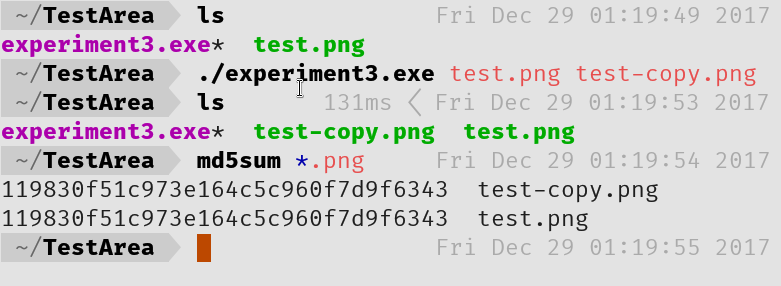
\includegraphics[width=0.8\linewidth]{exp3TestResult.png}
    \caption{测试过程及结果}
    \label{fig:exp3TestResult}
\end{figure}

\subsection{结果分析}
\label{sub:jie_guo_fen_xi_3}
从图\ref{fig:exp3TestResult}中可以看出,文件成功地被复制并且复制前后文件的内容是相同的,说明文件复制功能正常。同时这也说明了线程之间能够通过共享内存区传递信息、以及环形缓冲区能够有效的传递信息。

% Chapter 4 %%%%%%%%%%%%%%%%%
%%%%%%%%%%%%%%%%%%%%%%%%%%%%%

\chapter{Linux文件目录}
\label{cha:linuxwen_jian_mu_lu_4}

\section{实验目的}
\label{sec:shi_yan_mu_de_4}

\begin{enumerate}
    \item 了解Linux文件系统与目录操作;
    \item 了解Linux文件系统目录结构;
    \item 掌握文件和目录的程序设计方法。
\end{enumerate}

\section{实验内容}
\label{sec:shi_yan_nei_rong_4}

编程实现目录查询功能:\par
功能类似ls -lR;\par
查询指定目录下的文件及子目录信息:显示文件的类型、大小、时间等信息;\par
递归显示子目录中的所有文件信息。\par

\section{实验设计}
\label{sec:shi_yan_she_ji_4}

\subsection{总体设计}
\label{sub:zong_ti_she_ji_4}

通过Linux目录以及文件信息的接口,打印当前目录下的内容,并递归地调用这个程序打印这个目录所有子目录下的内容。首先研究ls -lR的输出规则,然后使用相似的规则进行输出。

\subsection{详细设计}
\label{sub:xiang_xi_she_ji_4}

本程序由三个函数构成:主函数main,负责递归的函数printDir以及负责打印目录和文件的函数printEntry。主函数负责调用printDir,printDir递归调用自身并在每次递归时调用printDir打印目录下的内容。程序的逻辑较为简单但细节部分较为复杂。ls -lR命令具有如下特征:
\begin{enumerate}
    \item 首先打印传入参数所表示目录的名字以及其下的内容。若没有传入参数则默认为当前目录``.''。
    \item 对于每个目录的打印,首先打印其相对路径(相对于传入参数),第二行打印total <块大小>,且此块大小不是文件系统的块大小(解释见下),第三行以及之后的行用于打印目录下所有Entry的内容。
    \item ls -lR每个文件夹后跟的total所表示的块大小意义为:physical-blocks-in-use $\times$ physical-block-size $\div$ LS-BLOCK-SIZE这一参数,其中physical-block-size-in-use是文件占用的物理块的数量,physical-block-size是物理块的大小,而LS-BLOCK-SIZE是可以由ls的-{}-block-size参数指定的,若未指定则其值与ls的实现有关\footnote{https://stackoverflow.com/a/33730697}。在编写以及测试本程序的计算机上,physical-block-size是4096,LS-BLOCK-SIZE是1024,也就是说一个文件所占有的块数量至少为4且一定为4的整数倍。
    \item 对于每个目录下Entry内容的打印顺序是根据文件名进行排序的,且是按照当前的locale设置进行排序(类似strcoll)而不是直接按照字节进行排序(类似strcmp)。
    \item 每个Entry的信息打印顺序是权限-硬链接数量-拥有者-拥有组-大小(字节)-修改时间-文件名。每两项之间使用一个空格隔开,每项的长度都是由所有打印出的文件的这一项的最大长度决定的(即在同一目下每一目录项的同一属性打印长度都是一致的)。除了文件名外,所有项都是右对齐的,最后修改时间包含3到4项,具体规则见下。
    \item 文件的最后修改时间的打印规则是:以距离当前时间是否超过6个月作为分隔,超过6个月的只打印月份、日期以及年份。小于6个月的打印月份、日期、最后修改的小时数、分钟数。\footnote{https://www.gnu.org/software/coreutils/manual/coreutils.html\#Formatting-file-timestamps}
\end{enumerate}

\section{实验过程}
\label{sec:shi_yan_guo_cheng_4}

\subsection{开发环境}
\label{sub:kai_fa_huan_jing_4}

\begin{tabular}{r l}
    操作系统 & Archlinux x86\_64 \\
    编译器 & gcc 7.2.1 \\
    自动编译 & GNU Make 4.2.1 \\
\end{tabular}

\subsection{实验步骤}
\label{sub:shi_yan_bu_zou_4}

首先编写代码,然后编译得到可执行文件experiment4.exe(编译选项与实验一相同),然后对于任一目录执行命令./experiment4.exe <目录名>,。再使用ls -lR对同一个目录进行操作并对比两个程序的输出。首先对于一个简单的目录进行测试,两个程序的输出结果如图\ref{fig:exp4Result}所示(在bash下运行)。

\begin{figure}[ht]
    \centering
    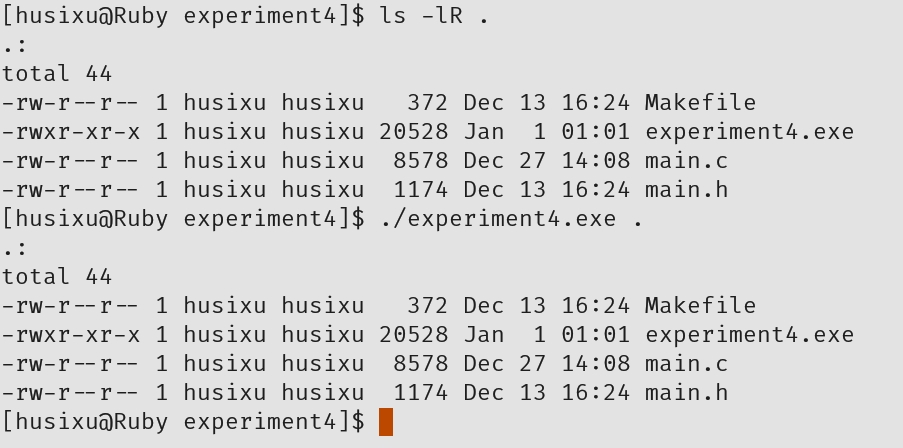
\includegraphics[width=0.8\linewidth]{exp4Result.png}
    \caption{简单目录实验结果}
    \label{fig:exp4Result}
\end{figure}

然后对于一个较为复杂的,有层级关系的目录进行测试,直接使用diff比较两个程序的输出,如图\ref{fig:exp4Result2}所示,可以看出,diff程序直接返回而没有任何输出,说明两个程序的输出结果是一致的。

\begin{figure}[ht]
    \centering
    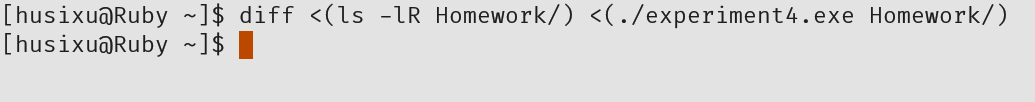
\includegraphics[width=0.8\linewidth]{exp4Result2.png}
    \caption{复杂目录实验结果}
    \label{fig:exp4Result2}
\end{figure}

\subsection{结果分析}
\label{sub:jie_guo_fen_xi_4}

图\ref{fig:exp4Result}以及\ref{fig:exp4Result2}所表示的结果表明,无论是否需要递归,exp4Result2都与ls -lR具有相同的输出。另外在测试中发现,对于大型目录(如/home或根目录等)experiment4.exe将由于栈溢出而崩溃,ls -lR则不会,这是由于experient4.exe是直接使用递归调用函数实现的,递归层数过深时会直接导致栈溢出,而ls则不是直接使用递归调用函数的方式遍历目录的。因此只能说在没有超过栈大小限制的情况下这一对目录进行操作的程序是有效的。

\appendix

\chapter{实验一代码}
\label{sec:shi_yan_yi_dai_ma_}
\noindent 头文件:
\inputCode[c]{../experiment1/main.h}
\noindent 实现文件:
\inputCode[c]{../experiment1/main.c}

\chapter{实验二代码}
\label{cha:shi_yan_er_dai_ma_}
\noindent 头文件:
\inputCode[c]{../experiment2/main.h}
\noindent 实现文件:
\inputCode[c]{../experiment2/main.c}

\chapter{实验三代码}
\label{cha:shi_yan_san_dai_ma_}
\noindent 头文件:
\inputCode[c]{../experiment3/main.h}
\noindent 实现文件:
\inputCode[c]{../experiment3/main.c}

\chapter{实验四代码}
\label{cha:shi_yan_si_dai_ma_}
\noindent 头文件:
\inputCode[c]{../experiment4/main.h}
\noindent 实现文件:
\inputCode[c]{../experiment4/main.c}


\vfill
{\tiny written by HuSixu \hfill powered by \XeLaTeX .}
\end{document}


